\documentclass[10pt]{beamer}
% Try building with xelatex instead of pdflatex

% These fonts can be removed if you don't want to use them.
\usepackage[T1]{fontenc}
\usepackage{FiraSans}
\usepackage{FiraMono}

% Metropolis theme - modern, minimal design
\usetheme[progressbar=frametitle]{metropolis}
\usepackage{appendixnumberbeamer}

% Professional tables
\usepackage{booktabs}

% Creative Commons icons
\usepackage[scale=2]{ccicons}

% Plotting
\usepackage{pgfplots}
\usepgfplotslibrary{dateplot}

% Smart spacing after custom commands
\usepackage{xspace}
\newcommand{\themename}{\textbf{\textsc{metropolis}}\xspace}

% Document metadata
\title{Metropolis Theme Demo}
\subtitle{A modern Beamer theme}
\date{}
\author{Your Name}
\institute{Your Institution}

\begin{document}

\maketitle

\begin{frame}{Table of Contents}
    \setbeamertemplate{section in toc}[sections numbered]
    \tableofcontents
\end{frame}

%--------------------------------------------------
\section{Introduction}
%--------------------------------------------------

\begin{frame}[fragile]{The Metropolis Theme}
    The \themename theme provides a clean, modern look for presentations.

    Enable it with:
    \begin{verbatim}
    \documentclass{beamer}
    \usetheme{metropolis}
    \end{verbatim}

    The theme features:
    \begin{itemize}
        \item Minimal visual noise
        \item Progress bar in frame titles
        \item Clean typography
    \end{itemize}
\end{frame}

%--------------------------------------------------
\section{Elements}
%--------------------------------------------------

\begin{frame}{Typography}
    The theme provides sensible defaults:

    \begin{itemize}
        \item Regular text for normal content
        \item \emph{Emphasized} text for stress
        \item \alert{Alerted} text for important points
        \item \textbf{Bold} for strong emphasis
    \end{itemize}
\end{frame}

\begin{frame}{Lists in Columns}
    \begin{columns}[T,onlytextwidth]
        \column{0.5\textwidth}
        \textbf{Bullet Points}
        \begin{itemize}
            \item Stocks
            \item Bonds
            \item Real Estate
        \end{itemize}

        \column{0.5\textwidth}
        \textbf{Numbered}
        \begin{enumerate}
            \item Identify risk
            \item Measure exposure
            \item Hedge position
        \end{enumerate}
    \end{columns}
\end{frame}

\begin{frame}{Tables}
    \begin{table}
        \caption{Asset Class Returns}
        \begin{tabular}{lrr}
            \toprule
            Asset & Return & Volatility \\
            \midrule
            Equities & 10.5\% & 18.2\% \\
            Bonds & 4.2\% & 5.1\% \\
            Commodities & 6.8\% & 22.4\% \\
            \bottomrule
        \end{tabular}
    \end{table}
\end{frame}

\begin{frame}{Blocks}
    Three block styles are available:

    \begin{columns}[T,onlytextwidth]
        \column{0.5\textwidth}
        \begin{block}{Default Block}
            Standard information.
        \end{block}

        \begin{alertblock}{Alert Block}
            Important warning.
        \end{alertblock}

        \column{0.5\textwidth}
        \begin{exampleblock}{Example Block}
            Illustrative content.
        \end{exampleblock}

        \metroset{block=fill}
        \begin{block}{Filled Block}
            With background.
        \end{block}
    \end{columns}
\end{frame}

%--------------------------------------------------
\section{Mathematics}
%--------------------------------------------------

\begin{frame}{Mathematical Content}
    The CAPM equation:
    \begin{equation*}
        E[R_i] = R_f + \beta_i (E[R_m] - R_f)
    \end{equation*}

    Black-Scholes option pricing:
    \begin{equation*}
        C = S_0 N(d_1) - K e^{-rT} N(d_2)
    \end{equation*}

    where:
    \[
        d_1 = \frac{\ln(S_0/K) + (r + \sigma^2/2)T}{\sigma\sqrt{T}}
    \]
\end{frame}

%--------------------------------------------------
\section{Graphics}
%--------------------------------------------------

\begin{frame}{Line Plots with PGFPlots}
    \begin{figure}
        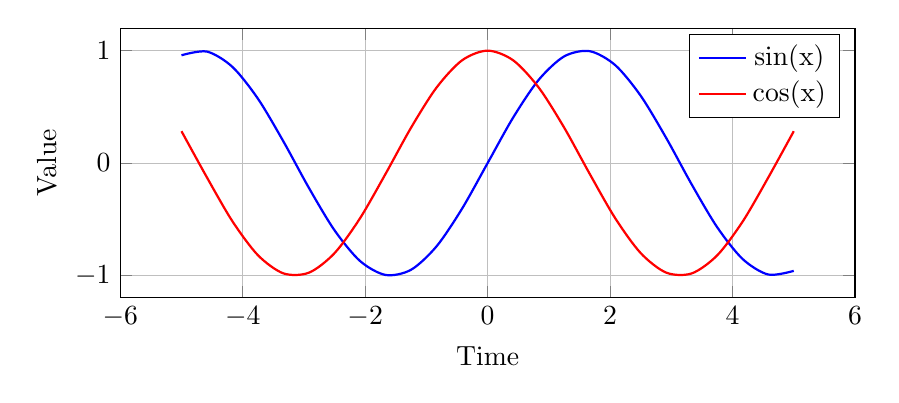
\begin{tikzpicture}
            \begin{axis}[
                width=0.9\textwidth,
                height=5cm,
                xlabel={Time},
                ylabel={Value},
                grid=major,
            ]
            \addplot[smooth, thick, blue] {sin(deg(x))};
            \addplot[smooth, thick, red] {cos(deg(x))};
            \legend{sin(x), cos(x)}
            \end{axis}
        \end{tikzpicture}
    \end{figure}
\end{frame}

\begin{frame}{Bar Charts}
    \begin{figure}
        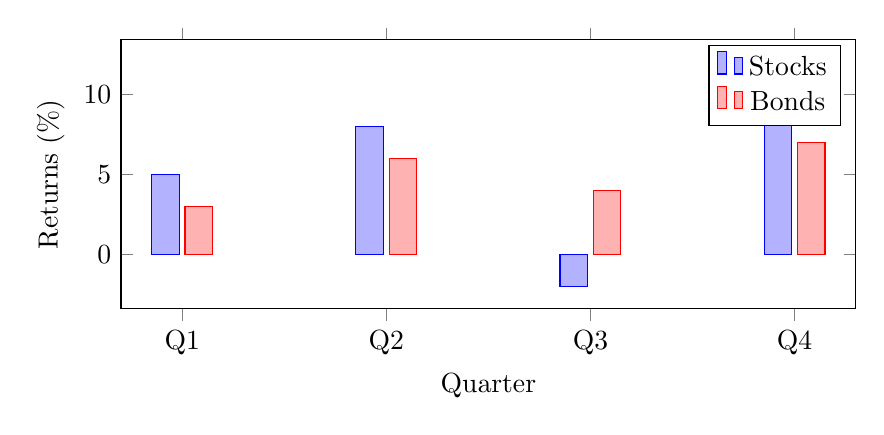
\begin{tikzpicture}
            \begin{axis}[
                ybar,
                width=0.9\textwidth,
                height=5cm,
                xlabel={Quarter},
                ylabel={Returns (\%)},
                symbolic x coords={Q1, Q2, Q3, Q4},
                xtick=data,
            ]
            \addplot coordinates {(Q1, 5) (Q2, 8) (Q3, -2) (Q4, 12)};
            \addplot coordinates {(Q1, 3) (Q2, 6) (Q3, 4) (Q4, 7)};
            \legend{Stocks, Bonds}
            \end{axis}
        \end{tikzpicture}
    \end{figure}
\end{frame}

%--------------------------------------------------
\section{Conclusion}
%--------------------------------------------------

\begin{frame}{Summary}
    The Metropolis theme provides:

    \begin{itemize}
        \item Clean, professional aesthetics
        \item Progress indicators
        \item Flexible block styles
        \item Full mathematical support
        \item Integrated plotting
    \end{itemize}

    \vspace{0.5cm}
    Get it at: \url{github.com/matze/mtheme}
\end{frame}

{\setbeamercolor{palette primary}{fg=black, bg=yellow}
\begin{frame}[standout]
    Questions?
\end{frame}
}

%--------------------------------------------------
\appendix
%--------------------------------------------------

\begin{frame}[fragile]{Backup Slides}
    The \verb|\appendix| command starts backup slides.

    With \verb|appendixnumberbeamer|, these slides don't count
    toward the total slide count.

    Use backup slides for:
    \begin{itemize}
        \item Additional details
        \item Anticipated questions
        \item Extended derivations
    \end{itemize}
\end{frame}

\begin{frame}[allowframebreaks]{References}
    \bibliography{bibliography}
    \bibliographystyle{abbrv}
\end{frame}

\end{document}
